\documentclass[preview]{standalone}

\usepackage{amsmath}
\usepackage{amssymb}
\usepackage{bettelini}
\usepackage{stellar}
\usepackage[version=4]{mhchem}
\usepackage{pgfplots}
\pgfplotsset{compat=1.17}

\hypersetup{
    colorlinks=true,
    linkcolor=black,
    urlcolor=blue,
    pdftitle={Stellar},
    pdfpagemode=FullScreen,
}

\begin{document}

\id{chimica-termodinamica-chimica-esercizi}
\genpage

\section{Esercizi termodinamica}

\begin{snippetexercise}{effetto-equilibrio-ex}{Spiega l'effetto ottenuto sull'equilibrio da una reazione}
    \[ O_{2(\text{g})} + N_{2(\text{g})} \rightleftharpoons 2NO_{2(\text{g})} \]
    \begin{itemize}
        \item \textbf{aumento della temperatura:}
            se la reazione diretta è endotermica, scaldare favorirà la produzione di prodotti,
            mentre se la reazione è esotermica, raffreddare favorirà la formazione di prodotti;
            ci sono due moli di gas sia a destra che a sinistra, per cui non abbiamo nessun influsso.
        \item \textbf{aumento della concentrazione di ossigeno:}
            viene favorita la produzione di prodotti (spostamento verso destra);
        \item \textbf{diminuzione pressione parziale di N\({}_2\):}
            viene diminuita la concentrazione di azoto, e per cui avremo meno prodotti;
        \item \textbf{aumento della concentrazione NO:}
            aumentano i reagenti (viene favorita la reazione inversa);
        \item \textbf{presenza di un catalizzatore:}
            l'equilibrio non cambia.
    \end{itemize}
\end{snippetexercise}

\begin{snippetexercise}{problema-concentrazione-chatelier-ex}{Problema concdentrazioni Le Chatelier}
    Alle condizioni standard di temperatura \(T=25^\circ C\) e di pressione
    \(p=1\) bar, in un recipiente rigido chiuso viene raggiunto il seguente equilibrio in fase gassosa:
    \begin{align*}
        2\text{CH}_{4(\text{g})} \leftrightharpoons \text{C}_2\text{H}_{2(\text{g})} + 3\text{H}_{2(\text{g})}
    \end{align*}
    La reazione diretta dell'equilibrio (1), comporta l'assorbimento di energia attraverso calore
    pari a 377 kJ per moli di C\({}_2\)H\({}_2\) prodotti.
    \\\\
    Il seguente grafico mostra le concentrazioni delle tre sostanze a formare la miscela gassosa racchiusa nel recipiente.
    \\
    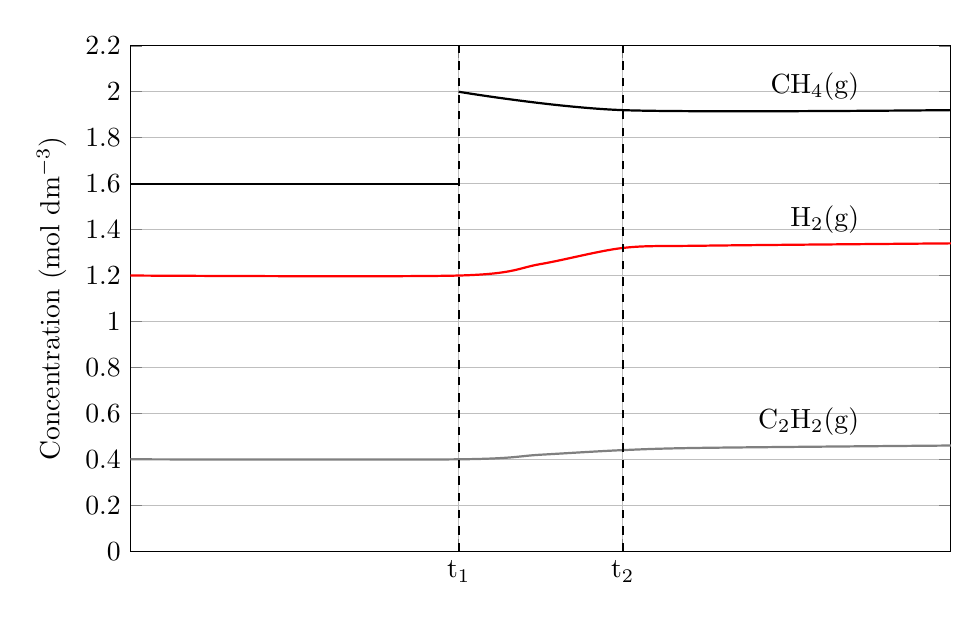
\begin{tikzpicture}
        \begin{axis}[
            width=12cm,
            height=8cm,
            xlabel={},
            ylabel={Concentration (mol dm$^{-3}$)},
            grid=major,
            xmin=0, xmax=10,
            ymin=0, ymax=2.2,
            xtick={4,6},
            xticklabels={t$_1$, t$_2$},
            ytick={0,0.2,...,2.2},
        ]
        
        % CH4(g) line before t1
        \addplot[thick, black, smooth] coordinates {
            (0, 1.6) (4, 1.6)
        };
    
        % CH4(g) line after t1
        \addplot[thick, black, smooth] coordinates {
            (4, 2.0) (6, 1.92) (10, 1.92)
        };
        
        % H2(g) line
        \addplot[thick, red, smooth] coordinates {
            (0, 1.2) (4, 1.2) (5, 1.25) (6, 1.32) (7, 1.33) (10, 1.34)
        };
        
        % C2H2(g) line
        \addplot[thick, gray, smooth] coordinates {
            (0, 0.4) (4, 0.4) (5, 0.42) (6, 0.44) (7, 0.45) (10, 0.46)
        };
        
        % Line at t1
        \draw[dashed, thick] (axis cs:4,0) -- (axis cs:4,2.2);
        
        % Line at t2
        \draw[dashed, thick] (axis cs:6,0) -- (axis cs:6,2.2);
    
        % Annotations for chemical compounds
        \node at (axis cs:9, 1.92) [anchor=south east] {CH$_4$(g)};
        \node at (axis cs:9, 1.34) [anchor=south east] {H$_2$(g)};
        \node at (axis cs:9, 0.46) [anchor=south east] {C$_2$H$_2$(g)};
        
        \end{axis}
    \end{tikzpicture}
    \begin{enumerate}
        \item Formulare l'espressione della legge dell'azione di massa per l'equilibrio (1) e determinare quindi il valore della costante di equilibrio \(K_{eq}\) a \(T=25^\circ C\):
            \[ \frac{0.4 \cdot {1.2}^3}{{1.6}^2} \approx 0.27 \]
        \item Nell'istante \(t=t_1\), viene introdotta una certa quantità di CH\({}_4\).
            Disegna l'andamento sul grafico di C\({}_2\)H\({}_2\), una volta raggiunto il nuovo equilibrio a \(t=t_2\):
            Dato che l'idrogeno aumenta di 0.12 moli, l'etino aumenta di 0.04 visto che il coefficiente stechiometrico
            dell'idrogeno è 3. Arriva quindi alla concentrazione di 0.44.
        \item Verso quale direzione si sposterebbe il sistema chimico (1) se la miscela gassosa inizialmente all'equilibrio venisse raffreddata?
            Raffreddare il sistema significa togliere energia, ossia calore termico. La reazione endotermica
            sfrutta energia termica per produrre i prodotti dai reagenti. Per il principio di Le Chatelier,
            dopo aver tolto del calore al sistema, il sistema si deve riequilibrare minimizzando la perturbazione.
            Per fare ciò il sistema deve produrre calore, e quindi favorirà la reazione inversa che produce calore (reagenti verso prodotti).
            Di conseguenza, si sposta verso sinistra.
    \end{enumerate}
\end{snippetexercise}

\end{document}
